\subsubsection{Activity Diagram - Quản lý tổ chức}



\begin{figure}[H]
    \centering
    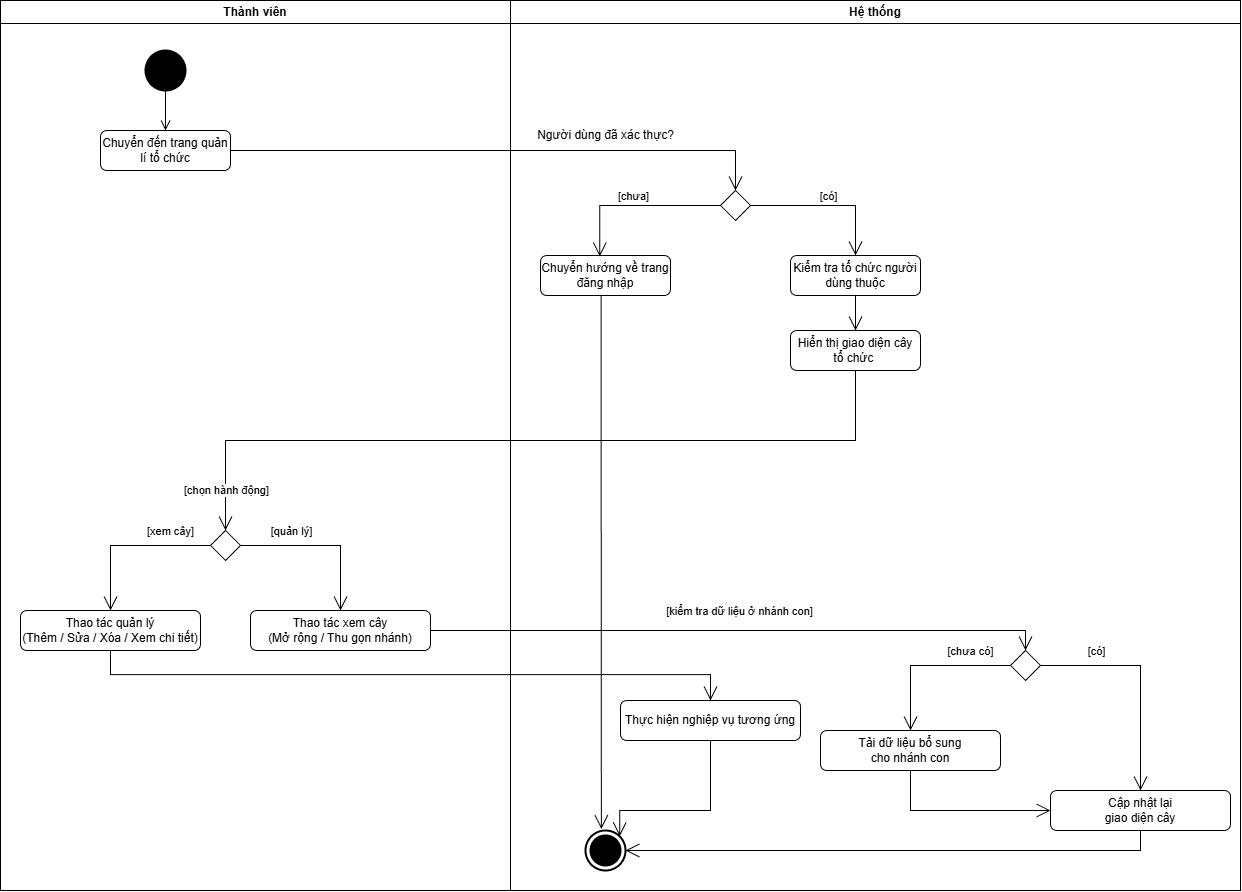
\includegraphics[width=1.0\textwidth]{Images/activity-diagram/activity_organization.drawio.png}
    \vspace{0.5cm}
    \caption{Activity Diagram - Quản lý tổ chức}
    \label{fig:act_org}
\end{figure}
Biểu đồ hoạt động tại Hình \ref{fig:act_org} mô tả luồng tương tác nghiệp vụ trên trang Quản lý tổ chức. Quy trình này không chỉ bao gồm các thao tác quản lý dữ liệu (CRUD) mà còn thể hiện chi tiết cơ chế tối ưu hóa trải nghiệm người dùng thông qua việc tải dữ liệu cây phân cấp theo nhu cầu.
Quy trình được chia thành hai làn xử lý (\textit{Swimlanes}) là \textbf{Thành viên} và \textbf{Hệ thống}, bao gồm các giai đoạn chính sau:

\paragraph{Khởi tạo và Kiểm soát truy cập}
Khi người dùng truy cập vào trang, hệ thống thực hiện chuỗi kiểm tra tự động trước khi hiển thị dữ liệu:
\begin{itemize}
    \item \textbf{Xác thực người dùng:} Hệ thống kiểm tra trạng thái đăng nhập. Nếu chưa xác thực, người dùng bị chuyển hướng về trang Đăng nhập.
    \item \textbf{Khởi tạo ngữ cảnh:} Nếu đã xác thực, hệ thống thực hiện bước \textit{"Kiểm tra tổ chức người dùng thuộc"}. Bước này giúp hệ thống xác định và ưu tiên hiển thị các đơn vị mà người dùng đang là thành viên lên đầu danh sách, sau đó mới hiển thị giao diện cây tổ chức hoàn chỉnh.
\end{itemize}

\paragraph{Phân loại hành động người dùng}
Tại giao diện chính, người dùng có thể thực hiện hai nhóm tác vụ, dẫn đến hai nhánh xử lý riêng biệt:
\begin{itemize}
    \item \textbf{Nhánh Quản lý (CRUD):} Bao gồm các thao tác Thêm, Sửa, Xóa hoặc Xem chi tiết. Hệ thống sẽ tiếp nhận và thực hiện các nghiệp vụ backend tương ứng rồi kết thúc luồng.
    \item \textbf{Nhánh Xem cây (View Tree):} Bao gồm thao tác Mở rộng (+) hoặc Thu gọn (-) các nhánh con của cây tổ chức.
\end{itemize}

\paragraph{Cơ chế hiển thị và Lazy Loading}
Khi người dùng chọn thao tác \textbf{Mở rộng nhánh} (thuộc nhóm thao tác xem cây), hệ thống áp dụng thuật toán tối ưu hóa dữ liệu:
\begin{enumerate}
    \item \textbf{Kiểm tra dữ liệu cục bộ:} Hệ thống kiểm tra xem dữ liệu của nhánh con đó đã được tải về trình duyệt chưa (\textit{Client-side Check}).
    \item \textbf{Quyết định tải dữ liệu:}
    \begin{itemize}
        \item \textit{Trường hợp chưa có (Cache Miss):} Hệ thống thực hiện hành động \textit{"Tải dữ liệu bổ sung cho nhánh con"} từ máy chủ.
        \item \textit{Trường hợp đã có (Cache Hit):} Hệ thống bỏ qua bước tải mạng và sử dụng ngay dữ liệu có sẵn.
    \end{itemize}
    \item \textbf{Cập nhật giao diện:} Cuối cùng, hệ thống cập nhật lại hiển thị cây (\textit{Re-render}) để mở rộng nhánh mà người dùng vừa chọn.
\end{enumerate}
